\documentclass[aspectratio=169]{beamer}

% Custom Futuristic Dark Theme
\usepackage{tikz}
\usepackage{xcolor}
\usepackage{listings}

% Define custom colors
\definecolor{DeepBackground}{HTML}{0B0E14}
\definecolor{NeonCyan}{HTML}{00F0FF}
\definecolor{NeonPurple}{HTML}{7000FF}
\definecolor{OffWhite}{HTML}{E2E8F0}
\definecolor{GrayAccent}{HTML}{1F2937}

% Code Listing Style
\lstdefinestyle{mystyle}{
    backgroundcolor=\color{GrayAccent},   
    commentstyle=\color{NeonCyan},
    keywordstyle=\color{NeonPurple},
    numberstyle=\tiny\color{OffWhite},
    stringstyle=\color{NeonCyan},
    basicstyle=\ttfamily\footnotesize\color{OffWhite},
    breaklines=true,                 
    captionpos=b,                    
    keepspaces=true,                 
    showspaces=false,                
    showstringspaces=false,
    showtabs=false,                  
    tabsize=2
}
\lstset{style=mystyle}

% Beamer Theme Settings
\mode<presentation>{
    \usetheme{default}
    \setbeamercolor{background canvas}{bg=DeepBackground}
    \setbeamercolor{normal text}{fg=OffWhite}
    \setbeamercolor{title}{fg=NeonCyan}
    \setbeamercolor{subtitle}{fg=OffWhite}
    \setbeamercolor{frametitle}{fg=NeonCyan, bg=DeepBackground}
    \setbeamercolor{structure}{fg=NeonCyan}
    \setbeamercolor{itemize item}{fg=NeonPurple}
    \setbeamercolor{itemize subitem}{fg=NeonCyan}
    \setbeamercolor{itemize subsubitem}{fg=OffWhite}
    
    % Fonts
    \setbeamerfont{title}{size=\huge, series=\bfseries}
    \setbeamerfont{subtitle}{size=\Large, series=\bfseries}
    \setbeamerfont{frametitle}{size=\LARGE, series=\bfseries}
    
    \setbeamertemplate{navigation symbols}{}
    
    % Custom Frame Title with a neon line
    \setbeamertemplate{frametitle}{
        \vspace{0.5cm}
        \usebeamerfont{frametitle}\insertframetitle
        \vspace{0.1cm}
        
\begin{tikzpicture}
            \draw[NeonCyan, thick] (0,0) -- (\textwidth, 0);
        \end{tikzpicture}
    }
}

\title{Big Data Analytics of Crime Patterns}
\subtitle{\textcolor{NeonPurple}{using Hadoop MapReduce and Apache Hive}}
\author[Group Name]{Your Group Members}
\institute[Amrita]{Amrita Vishwa Vidyapeetham}
\date{\today}

\begin{document}

% Slide 1: Title Page
\begin{frame}
    \begin{tikzpicture}[remember picture,overlay]
        \fill[DeepBackground] (current page.south west) rectangle (current page.north east);
        \draw[NeonCyan, thick, opacity=0.3] (current page.north west) -- (current page.south east);
        \draw[NeonPurple, thick, opacity=0.3] (current page.south west) -- (current page.north east);
        \fill[NeonCyan] (current page.south west) circle (1cm);
        \fill[NeonPurple] (current page.north east) circle (1.5cm);
    \end{tikzpicture}
    \vspace{2cm}
    \begin{center}
        \usebeamerfont{title}\textcolor{NeonCyan}{\inserttitle}\par
        \vspace{0.5cm}
        \usebeamerfont{subtitle}\insertsubtitle\par
        \vspace{1cm}
        \textit{\insertauthor} \\
        \vspace{0.5cm}
        \insertinstitute
    \end{center}
\end{frame}

% Slide 2: Agenda
\begin{frame}{Agenda}
    \begin{itemize}
        \item Introduction \& Motivation
        \item Problem Statement
        \item Dataset Description
        \item Architecture Pipeline
        \item Hadoop MapReduce Implementation
        \item Apache Hive Analytics
        \item Execution Results
        \item Conclusion
    \end{itemize}
\end{frame}

% Slide 3: Introduction
\begin{frame}{Introduction}
    \begin{itemize}
        \item The rise of Big Data provides an unprecedented opportunity to analyze public safety records.
        \item City crime records encompass millions of rows of incidents, locations, dates, and types.
        \item Processing this data efficiently requires distributed frameworks.
        \item We leverage \textbf{\textcolor{NeonCyan}{Hadoop MapReduce}} for raw parallel processing and \textbf{\textcolor{NeonPurple}{Apache Hive}} for SQL-based analytical querying.
    \end{itemize}
\end{frame}

% Slide 4: Motivation
\begin{frame}{Motivation}
    \textbf{Why analyze crime data?}
    \vspace{0.3cm}
    \begin{itemize}
        \item \textbf{Public Safety:} Identifying high-crime zones helps improve community security.
        \item \textbf{Resource Allocation:} Enables police departments to deploy patrols dynamically based on historical hotspots.
        \item \textbf{Trend Forecasting:} Predicting the frequency and nature of crimes across different districts and timeframes.
        \item \textbf{Big Data Challenge:} Traditional RDBMS fail to scale efficiently with millions of such rows.
    \end{itemize}
\end{frame}

% Slide 5: Problem Statement
\begin{frame}{Problem Statement}
    \begin{center}
        \Large \textit{"To design and implement a scalable Big Data pipeline that can ingest, process, and extract actionable intelligence from massive real-world crime datasets."}
    \end{center}
    \vspace{0.5cm}
    \textbf{Objectives:}
    \begin{itemize}
        \item Demonstrate a complete data pipeline from HDFS storage to advanced analytics.
        \item Perform category-wise statistics using MapReduce.
        \item Execute 10 meaningful complex queries utilizing aggregations, filtering, and joins in Hive.
    \end{itemize}
\end{frame}

% Slide 6: Dataset Overview
\begin{frame}{Dataset Overview}
    \textbf{Dataset:} Chicago Crimes (2001 to Present)\\
    \vspace{0.2cm}
    \begin{itemize}
        \item \textbf{Scope:} Extracts real-world incident reports from the Chicago Data Portal.
        \item \textbf{Size:} 10,000 recent records processed for this demonstration.
        \item \textbf{Key Features:}
        \begin{itemize}
            \item \textcolor{NeonCyan}{Identifiers:} \texttt{id}, \texttt{case\_number}, \texttt{date}
            \item \textcolor{NeonCyan}{Categories:} \texttt{primary\_type}, \texttt{description}
            \item \textcolor{NeonCyan}{Location:} \texttt{district}, \texttt{ward}, \texttt{community\_area}
            \item \textcolor{NeonCyan}{Flags:} \texttt{arrest}, \texttt{domestic}
        \end{itemize}
    \end{itemize}
\end{frame}

% Slide 7: Preprocessing & Storage
\begin{frame}{Data Preprocessing \& HDFS Storage}
    \textbf{Preprocessing Phase:}
    \begin{itemize}
        \item Raw CSV files often contain embedded newlines within quotes.
        \item We implemented a Python script to clean these records, ensuring perfect compatibility with Hadoop's \texttt{TextInputFormat}.
    \end{itemize}
    \vspace{0.3cm}
    \textbf{HDFS Storage:}
    \begin{itemize}
        \item Dataset uploaded to HDFS distributed storage.
        \item Command: \texttt{hdfs dfs -put chicago\_crimes.csv /user/crimes/}
    \end{itemize}
\end{frame}

% Slide 8: Architecture
\begin{frame}{System Architecture}
    \begin{center}
        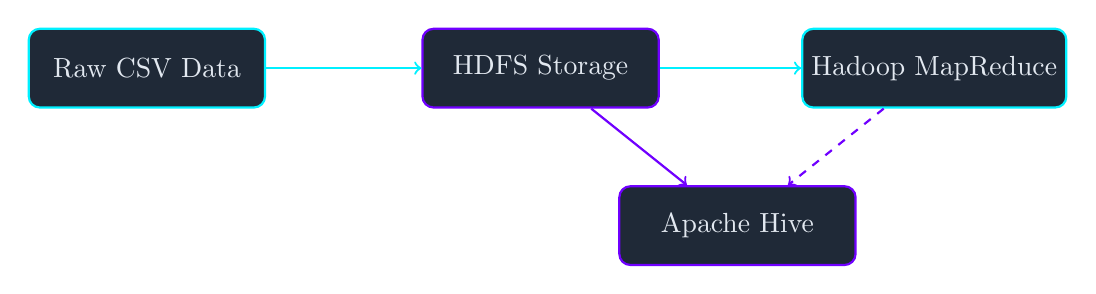
\begin{tikzpicture}
            % A simple flowchart for the architecture
            \node[draw=NeonCyan, thick, fill=GrayAccent, text=OffWhite, minimum width=3cm, minimum height=1cm, rounded corners] (A) at (0,3) {Raw CSV Data};
            \node[draw=NeonPurple, thick, fill=GrayAccent, text=OffWhite, minimum width=3cm, minimum height=1cm, rounded corners] (B) at (5,3) {HDFS Storage};
            \node[draw=NeonCyan, thick, fill=GrayAccent, text=OffWhite, minimum width=3cm, minimum height=1cm, rounded corners] (C) at (10,3) {Hadoop MapReduce};
            \node[draw=NeonPurple, thick, fill=GrayAccent, text=OffWhite, minimum width=3cm, minimum height=1cm, rounded corners] (D) at (7.5,1) {Apache Hive};
            
            \draw[->, NeonCyan, thick] (A) -- (B);
            \draw[->, NeonCyan, thick] (B) -- (C);
            \draw[->, NeonPurple, thick] (B) -- (D);
            \draw[->, NeonPurple, thick, dashed] (C) -- (D);
        \end{tikzpicture}
    \end{center}
    \vspace{0.5cm}
    \begin{itemize}
        \item Centralized data lake on HDFS.
        \item MapReduce for low-level transformations.
        \item Hive for structured intelligence gathering.
    \end{itemize}
\end{frame}

% Slide 9: MapReduce Overview
\begin{frame}{Hadoop MapReduce Implementation}
    \textbf{Problem:} Calculate the total occurrences of each Crime Type.\\
    \vspace{0.3cm}
    \textbf{Mapper Logic:}
    \begin{itemize}
        \item Input: \texttt{(ByteOffset, Line of text)}
        \item Ignores CSV headers.
        \item Splits line correctly handling commas within double quotes.
        \item Extracts the 6th column (\texttt{primary\_type}).
        \item Output: \texttt{(CrimeType, 1)}
    \end{itemize}
\end{frame}

% Slide 10: MapReduce Code
\begin{frame}[fragile]{MapReduce: Reducer Logic}
    \textbf{Reducer Logic:}
    \begin{itemize}
        \item Input: \texttt{(CrimeType, [1, 1, 1, ...])}
        \item Sums up all the '1's for a given crime type.
        \item Output: \texttt{(CrimeType, Total\_Count)}
    \end{itemize}
    \vspace{0.3cm}
    \begin{lstlisting}[language=Java]
public void reduce(Text key, Iterable<IntWritable> values, Context context) {
    int sum = 0;
    for (IntWritable val : values) {
        sum += val.get();
    }
    result.set(sum);
    context.write(key, result);
}
    \end{lstlisting}
\end{frame}

% Slide 11: MapReduce Results
\begin{frame}{MapReduce Execution \& Results}
    \begin{itemize}
        \item Successfully packaged as a JAR and executed on YARN.
        \item Processed 10,000 rows across mappers and reducers.
    \end{itemize}
    \vspace{0.3cm}
    \textbf{Sample Output (\texttt{part-r-00000}):}
    \begin{center}
        \texttt{THEFT \hspace{1cm} 2150} \\
        \texttt{BATTERY \hspace{1cm} 1857} \\
        \texttt{CRIMINAL DAMAGE \hspace{0.2cm} 1207} \\
        \texttt{ASSAULT \hspace{1cm} 905} \\
    \end{center}
\end{frame}

% Slide 12: Hive Setup
\begin{frame}{Apache Hive Analytics: Setup}
    \begin{itemize}
        \item Created an external table \texttt{crimes} mapping directly to HDFS data.
        \item \textbf{Serialization/Deserialization:} Used \texttt{OpenCSVSerde} to properly parse fields enclosed in quotes containing commas.
        \item Created a secondary table \texttt{community\_areas} holding area codes and names to demonstrate table joins.
    \end{itemize}
\end{frame}

% Slide 13: Hive Queries 1
\begin{frame}{Hive Analytics: Basic Queries}
    \begin{itemize}
        \item \textbf{\textcolor{NeonCyan}{SELECT \& LIMIT:}} Retrieved incident IDs and descriptions.
        \item \textbf{\textcolor{NeonCyan}{WHERE clause:}} Filtered incidents resulting specifically in a narcotics arrest.
        \item \textbf{\textcolor{NeonCyan}{ORDER BY:}} Sorted severe cases like homicides by recency.
        \item \textbf{\textcolor{NeonCyan}{GROUP BY \& COUNT:}} Identified which locations (e.g., STREET, APARTMENT) experience the highest crime volumes.
    \end{itemize}
\end{frame}

% Slide 14: Hive Queries 2
\begin{frame}{Hive Analytics: Advanced Aggregations}
    \begin{itemize}
        \item \textbf{\textcolor{NeonCyan}{HAVING clause:}} Extracted major crime categories by filtering for counts $>$ 500.
        \item \textbf{\textcolor{NeonCyan}{SUM:}} Calculated the absolute total number of arrests made within each police district.
        \item \textbf{\textcolor{NeonCyan}{AVG:}} Analyzed the average rate of domestic-related crimes across different beats.
        \item \textbf{\textcolor{NeonCyan}{MAX \& MIN:}} Automatically pinpointed the highest and lowest crime districts.
        \item \textbf{\textcolor{NeonCyan}{JOIN:}} Combined the raw \texttt{crimes} data with \texttt{community\_areas} to print human-readable neighborhood names.
    \end{itemize}
\end{frame}

% Slide 15: Interpretation
\begin{frame}{Results \& Interpretation}
    \textbf{Key Insights Derived:}
    \vspace{0.3cm}
    \begin{itemize}
        \item \textbf{Property Crimes Dominant:} Theft and Battery make up the vast majority of incidents.
        \item \textbf{Location Vulnerabilities:} Streets and sidewalks are the most common locations for incidents.
        \item \textbf{Enforcement Efficacy:} Analyzing arrests via Hive shows significant variations in arrest rates across different crime types and districts.
    \end{itemize}
\end{frame}

% Slide 16: Conclusion
\begin{frame}{Conclusion}
    \begin{itemize}
        \item Successfully ingested and analyzed a large-scale real-world dataset.
        \item \textbf{\textcolor{NeonCyan}{MapReduce}} proved highly efficient for unstructured low-level data processing and aggregations.
        \item \textbf{\textcolor{NeonPurple}{Apache Hive}} demonstrated immense power for executing complex, relational-style queries on distributed files.
        \item This pipeline can scale to millions of records, providing an essential backbone for civic analytics.
    \end{itemize}
\end{frame}

% Slide 17: Q&A
\begin{frame}
    \begin{tikzpicture}[remember picture,overlay]
        \fill[DeepBackground] (current page.south west) rectangle (current page.north east);
        \draw[NeonCyan, thick] (current page.center) circle (3cm);
        \draw[NeonPurple, thick] (current page.center) circle (3.2cm);
    \end{tikzpicture}
    \begin{center}
        \vspace{1.5cm}
        \usebeamerfont{title}\textcolor{NeonCyan}{Q \& A}\par
        \vspace{0.5cm}
        Thank you for listening.\\
        \vspace{1cm}
        \textbf{\textcolor{NeonPurple}{Any Questions?}}
    \end{center}
\end{frame}

\end{document}
